\documentclass[10pt]{article}

\usepackage{amsthm}
\usepackage[toc,page]{appendix}
\usepackage{amssymb}
\usepackage{bm}
\usepackage{pslatex,palatino,avant,graphicx,color}
\usepackage{colortbl}
\usepackage{fullpage}
\usepackage{mathtools}
\usepackage{natbib}
\usepackage{amsmath}
\usepackage{caption}
%\usepackage{subfigure}
\usepackage{subcaption}
\usepackage{bm}
\usepackage{wrapfig}
\usepackage{enumerate}
\usepackage{rotating}
\usepackage{multirow}
\usepackage{tabularx}
\usepackage{tikz}
\usepackage{pgfplots}
\usepackage{bbm}
\usepackage[titles,subfigure]{tocloft} % Alter the style of the Table of Contents

\newtheorem{lemma}{Lemma}
%\pdfminorversion=4
% NOTE: To produce blinded version, replace "0" with "1" below.
\newcommand{\blind}{0}

% DON'T change margins - should be 1 inch all around.
\addtolength{\oddsidemargin}{0in}%
\addtolength{\evensidemargin}{0in}%
\addtolength{\textwidth}{0in}%
\addtolength{\textheight}{0in}%
\addtolength{\topmargin}{0in}%


\renewcommand{\cftsecfont}{\rmfamily\mdseries\upshape}
\renewcommand{\cftsecpagefont}{\rmfamily\mdseries\upshape} % No bold!

\newcommand{\indicator}[1]{\mathbbm{1}\left( #1 \right) }
\newcommand{\hb}{\hat{b}}
\newcommand{\ha}{\hat{a}}
\newcommand{\htheta}{\hat{\theta}}
\newcommand{\halpha}{\hat{\alpha}}
\newcommand{\hmu}{\hat{\mu}}
\newcommand{\hsigma}{\hat{\sigma}}
\newcommand{\hphi}{\hat{\phi}}
\newcommand{\htau}{\hat{\tau}}
\newcommand{\heta}{\hat{\eta}}
\newcommand{\E}[1]{\mbox{E}\left[#1\right]}
\newcommand{\Var}[1]{\mbox{Var}\left[#1\right]}
\newcommand{\Indicator}[1]{\mathbbm{1}_{ \left( #1 \right) } }
\newcommand{\dNormal}[3]{ N\left( #1 \left| #2, #3 \right. \right) }
\newcommand{\Beta}[2]{\mbox{Beta}\left( #1, #2 \right)}
\newcommand{\alphaphi}{\alpha_{\hphi}}
\newcommand{\betaphi}{\beta_{\hphi}}
\newcommand{\expo}[1]{ \exp\left\{ #1 \right\}}
\newcommand{\tauSquareDelta}{\htau^2
  \left(\frac{1-\expo{-2\htheta\Delta}}{2\htheta} \right)}
\newcommand{\mumu}{\mu_{\hmu}}
\newcommand{\sigmamu}{\sigma^2_{\hmu}}
\newcommand{\sigmamuexpr}{\log\left( \frac{\VarX}{\EX^2} + 1 \right)}
\newcommand{\mumuexpr}{\log(\EX) -  \log\left( \frac{\VarX}{\EX^2} + 1 \right) /2 }

\newcommand{\EX}{\mbox{E}\left[ X \right] }
\newcommand{\VarX}{\mbox{Var}\left[ X \right] }
\newcommand{\mueta}{\mu_{\heta} }
\newcommand{\sigmaeta}{\sigma^2_{\heta}}
\newcommand{\sigmaetaexpr}{ \log\left( \frac{\VarX}{\EX^2} + 1 \right) }
\newcommand{\muetaexpr}{ \log(\EX) -  \sigmaetaexpr /2 }

\newcommand{\mualpha}{\mu_{\halpha} }
\newcommand{\sigmaalpha}{\sigma^2_{\halpha}}
\newcommand{\sigmaalphaexpr}{ \log\left( \frac{\VarX}{\EX^2} + 1 \right) }
\newcommand{\mualphaexpr}{ \log(\EX) -  \sigmaalphaexpr /2 }

\newcommand{\mutauexpr}{ \frac{2}{T} \EX }
\newcommand{\sigmatauexpr}{ \frac{4}{T^2} \Var{X}}

\newcommand{\alphatau}{\alpha_{\htau^2}}
\newcommand{\betatau}{\beta_{\htau^2}}

\newcommand{\Gam}[2]{\mbox{Gamma}\left( #1, #2 \right) }
\newcommand{\InvGam}[2]{\mbox{Inv-Gamma}\left( #1, #2 \right) }

%%% END Article customizations

%%% The "real" document content comes below...

% \newbox{\LegendeA}
% \savebox{\LegendeA}{
%    (\begin{pspicture}(0,0)(0.6,0)
%    \psline[linewidth=0.04,linecolor=red](0,0.1)(0.6,0.1)
%    \end{pspicture})}
% \newbox{\LegendeB}
%    \savebox{\LegendeB}{
%    (\begin{pspicture}(0,0)(0.6,0)
%    \psline[linestyle=dashed,dash=1pt 2pt,linewidth=0.04,linecolor=blue](0,0.1)(0.6,0.1)
%    \end{pspicture})}

\title{A Range-Based Bivariate Stochastic Volatility Model: Towards Closed-Form Solution}
\author{Georgi Dinolov, Abel Rodriguez, Hongyun Wang}
\date{} % Activate to display a given date or no date (if empty),
         % otherwise the current date is printed

\begin{document}
\def\spacingset#1{\renewcommand{\baselinestretch}%
{#1}\small\normalsize} \spacingset{1}

\bigskip

\vspace{1cm}

In this chapter we develop an analytic solution to the normalized
problem for small $\tilde{\sigma}$ values. We illustrate our approach
with the simple case where $\rho=0$.

\subsection{A small-parameter analytic solution}
In the previous chapter we introduced a numerical solution that works
for relatively benign parameter ranges. However, the numerical
solution fails for small parameters of $(\tilde{\sigma},
\tilde{t})$. Here, we introduce an analytic solution that works for
certain small-$\tilde{\sigma}$.

\subsubsection{Illustration with $\rho=0$ and sufficiently small
  $\tilde{t}$}
Consider the normalized diffusion problem with $\rho=0$
\[
  \frac{\partial q}{\partial t} = \frac{1}{2}\frac{\partial^2 q}{\partial x^2} + \frac{1}{2}\tilde{\sigma}^2 \frac{\partial^2 q}{\partial y^2}.
\]
and an intial condition $(x_0, y_0)$ with absorbing boundaries on the
unit square. The fundamental solution to the problem is an
uncorrelated bivariate Gaussian with variances $t$ and
$t\tilde{\sigma}^2$ in the $x$ and $y$ directions, respectively. The
problem setup and a contour plot of the fundamental solution is
illustrated in Figure (\ref{fig:normalized-problem-rho-0}). As in
Chapter 2, we can scale, rotate, and scale again the problem, so that
the boundaries of the computational domain have changed, but the
fundamental solution to the problem is defined by an uncorrelated
bivariate Gaussian distribution with variance $t$ in each
direction. The transformed problem is shown in Figure
(\ref{fig:transformed-problem-rho-0}).

The topology under the transformed problem permits the fundamental
solution to be translated and rotated without violating the governing
PDE. Hence, we may reflect about the boundaries to enforce the
conditions there while producing a system of images whose sum
satisfies the PDE. In the $\rho=0$ case, the orthogonal angles between
adjecent boundaries ensure that none of the images that result from
repeated reflections fall within the computational domain. This
further allows for subsequent images for fall further from the domain
(scaling linearly in distance) so that we can numerically solve the
problem with a finite system of images.
\begin{figure}
  \centering
  %%
  %%
  \begin{tabular}{cc}
    \begin{minipage}{0.40\textwidth}
      \centering
      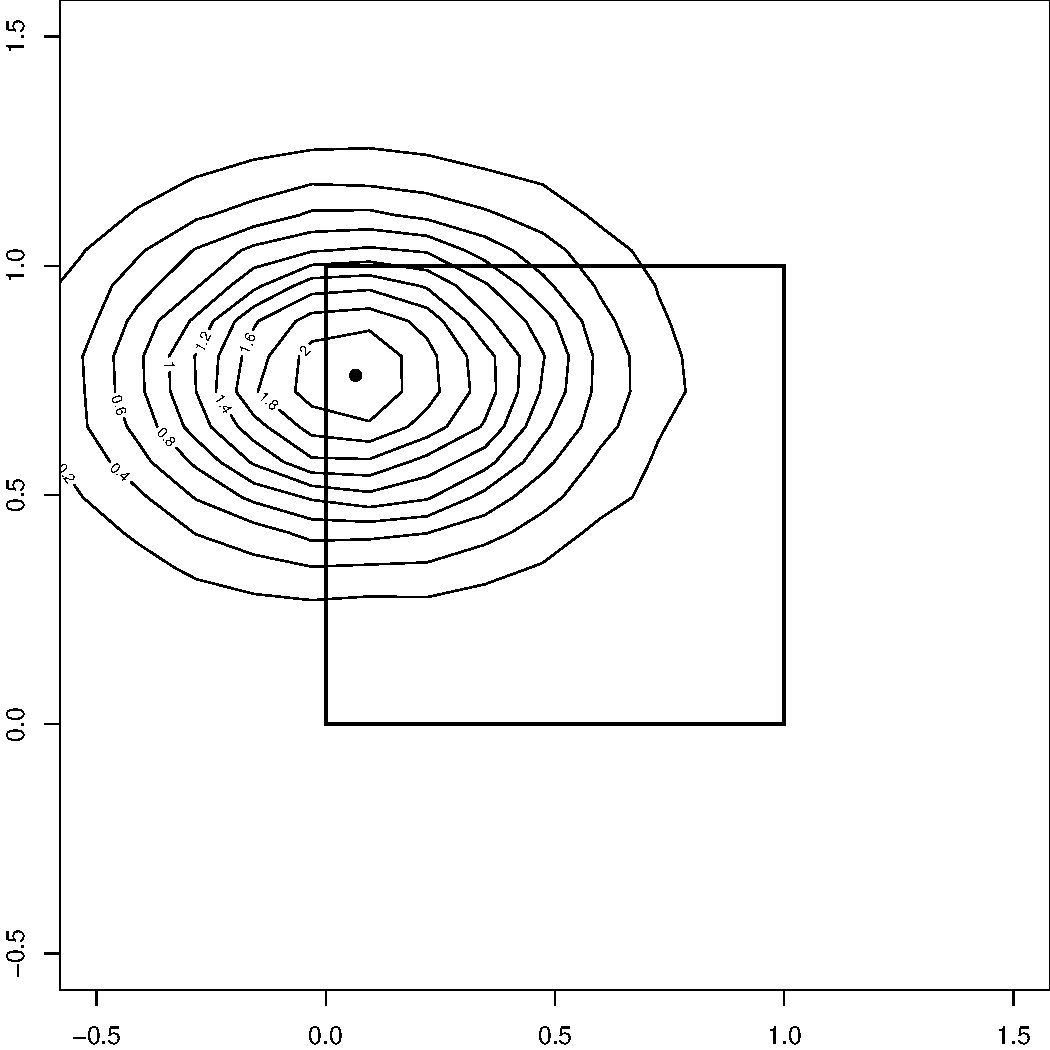
\includegraphics[width=1\linewidth]{illustration-rho-0-normalized.pdf}
      \caption{hello world}
      \label{fig:normalized-problem-rho-0}
    \end{minipage}
    %%
    & \begin{minipage}{0.40\textwidth}
      \centering
      \includegraphics[width=1\linewidth]{illustration-rho-0-transformed.pdf}
      \caption{Small time $\tilde{t} \approx 0.10$.}
      \label{fig:transformed-problem-rho-0}
    \end{minipage}
  \end{tabular}  
\end{figure}

However, instead of fully solving the problem, we can compose a system
of images by reflecting about each of the boundaries once and picking
the greatest possible time $\tilde{t}$ such that all boundaries are
either numerically or analytically enforced. There are at most 24 such
systems of images, not all of them unique and with different time
$\tilde{t}$, and each comprized of the fundamental solution
with a location parameter that is a function of the boundary
parameters. The solution to the PDE is of the form
\[
  \bar{q}(\xi, \eta, \tilde{t}) = \sum_{j=1}^J G(\xi,\eta, \tilde{t}| \xi_0^{(j)}(a_x, b_x, a_y, b_y), \eta_0^{(j)}(a_x, b_x, a_y, b_y)).
\]
Out of the $J=16$ images in each system, only one of the summands has
location parameters that are dependent on all four boundary parameters
(red), since only one image is the result of successive reflections
about each one of the boundaries.  Transforming back to the original
coordinate system and differentiating produces a solution for each
system
\[
  \frac{\partial^4 \bar{q}(x, y, \tilde{t})}{\partial a_x
    \partial b_x \partial a_y \partial b_y} = \frac{\partial^4
    G(x,y, \tilde{t}| \tilde{\sigma}, x_0^{(J)}(a_x, b_x, a_y, b_y),
    y_0^{(J)}(a_x, b_x, a_y, b_y))} {\partial a_x \partial b_x
    \partial a_y \partial b_y}.
\]
Since the analytic solution is unique, we can average the above
approximate soltions if we use a small $\tilde{t}$ that is valid for
more than one of the possible image configurations.

dependency of the Only one of the images in each system has,
therefore, a nonzero derivative with respect to all four
boundaries. Hence, the

For a sufficiently small $\tilde{t}$, we
can average the solutions, since the solution to the problem is
unique. 



note that for this
setup with $\tilde{\sigma} < 1$, the fundmental solution is
numerically zero on boundaries 1 and 3. Hence, we only need to enforce
boundaries 2 and 4, which can be done with a finite number of reflections.

Alternatively, we can scale $t$ down to acheive the same effect. 

Reflecting about 1 and 3 produces a system of images which satisfies
all boundaries and where at least one image has a non-zero fourth
order derivative with respect to the boundary parameters. Of course,
this is system of images is not unique, but we have shown that, by
either making $\tilde{\sigma}$ or $t$ small enough, we can produce an
analytic solution to the derivative problem. Next, we produce a
counterexample which shows that it is not always possible to scale $t$
down to achieve this.

\subsubsection{Counterexample with $\rho \neq 0$}
In the above illustration we saw how we can produce a system of images
that satisfies the problem equation at the boundaries either
numerically or analytically. Now we show a combination of parameters
that violates the problem if the method of images is used.

As in Chapter 2, we scale, rotate, and scale
again, so that the fundamental solution is $N(x,y|t)$. However, since
$\rho=0$, only the initial scaling is sufficient to perform
reflections. Thus, the effective problem domain is a rectangle of
height $1/\tilde{\sigma}$. We can pick a $\tilde{\sigma}$ small enough
such that the fundamental solution is numerically zero at boundaries 1
and 3 for $\tilde{t}$. Relfecting about boundaries 2 and 4 a finite
number of times is sufficient to enforce the boundaries. Reflecing about Now the fundamental solution is
$N(x,y|t)$. Reflecting about boundary 1 enforces the BC there. Then,
reflecting the system about boundary 2 enforces BC there, but the
additional images (labeled by 3 and red) disturb the condition at
boundary 1. Next, we can reflect the system about boundary 3, then 4,
where in each subsequent reflection we enforce the current boundary
and disturb the previous ones. However, the images

The approach we use to motivate the calculations for the
small-parameter solution is considering the problem with
$\rho=0$. Here we consider the normalized problme such that
$\tilde{\sigma} \leq 1$ and the diffusion problem is

Now consider a configuration of images generated by reflecting once
about each boundary. For a given $(\rho=0, \tilde{t})$, we can find a
sufficiently small $\tilde{\sigma}$ such that at least one of the 24
possible configurations satisfies the boundary conditions either
analytically or numerically. In this configuration, only one of the 16
images has a location parameter that is a function of all four
boundaries, and it is the only image that contributes to $\partial_{\Omega} q$. 


\end{document}